\documentclass[10pt]{article}
\usepackage[letterpaper,margin=0.53in]{geometry}
\usepackage{amsmath,amssymb,booktabs,array,graphicx,microtype,tikz,xcolor}
\usepackage[compact]{titlesec}
\usepackage[hidelinks]{hyperref}
\usepackage[numbers,sort&compress]{natbib}
\setlength{\parindent}{0pt}
\setlength{\parskip}{2.2pt}
\setlength{\tabcolsep}{4pt}
\renewcommand{\arraystretch}{1.08}
\titlespacing*{\section}{0pt}{5pt}{2pt}
\definecolor{softgreen}{RGB}{224,242,232}
\definecolor{hardred}{RGB}{244,218,214}
\title{\vspace{-1.5em}LanternTrace Physics, Resistance, and Grid Resolution\\\large A two-page explanation without assuming a physics background}
\author{Alex Dils}
\date{17 August 2026}

\begin{document}
\maketitle
\vspace{-1.6em}
\fontsize{9}{10.35}\selectfont

\begin{abstract}
LanternTrace moves a dimensionless \emph{relative establishment pressure} $u$ across a map; it does not estimate an insect count.  The revised model has no hand-tuned spread coefficients.  Its growth rate and natural-spread scale come from spotted-lanternfly studies, its diffusion coefficient is derived from those two values, and climate and terrain enter through an explicit resistance law.  Each cell-size setting is now an independent physics solve, so smaller cells mean higher numerical resolution rather than a prettier interpolation.
\end{abstract}
\vspace{-0.6em}

\begin{table}[h]
\centering
\caption{Constants and rules used by the current simulation.  Biological numbers have literature provenance; interface and normalization rules are identified rather than disguised as biological measurements.}
\label{tab:constants}
\scriptsize
\begin{tabular}{@{}p{0.20\linewidth}p{0.14\linewidth}p{0.58\linewidth}@{}}
\toprule
Quantity & Value & Basis and interpretation \\
\midrule
Maximum growth $r$ & $1.5~\mathrm{yr}^{-1}$ & Highest-recall growth setting in Ladin et al.'s lanternfly agent-based experiment; it is a published scenario value, not a measured fecundity constant \citep{ladin2023}. \\
Natural front scale $c$ & $25~\mathrm{km\,yr}^{-1}$ & Approximate maximum intrinsic annual spread estimated by the resistance-distance lanternfly study \citep{ruzzier2025}; diffusion-only spread was independently estimated as $25\pm11~\mathrm{km\,yr}^{-1}$ \citep{belouard2025}. \\
Diffusivity $D$ & $104.17~\mathrm{km^2\,yr}^{-1}$ & Derived, not tuned: $D=c^2/(4r)$ from the Fisher--KPP wave speed $c=2\sqrt{rD}$ \citep{fisher1937}. \\
Physics step $\Delta t$ & $1$ year & One full lanternfly generation; the species is univoltine and Ladin et al. use a one-year step \citep{ladin2023,wakie2020}. \\
Resistance baseline & $R=1$ & Definition of an ideal cell: climate $C=1$ and terrain permeability $G=1$.  Habitat-derived resistance follows the published resistance-distance approach \citep{ruzzier2025}. \\
Grid levels & $0.25,0.5,0.75,1^\circ$ & Numerical resolution ladder.  The finest cells are roughly $20$--$28$ km wide over the U.S., close to the published 20--25 km observation/spread scale \citep{zhao2024,ruzzier2025}; coarser levels are integer multiples for comparison. \\
Water boundary & $\leq50\%$ U.S. land $\Rightarrow u=0$ & User-specified display/domain rule, not a biological literature value.  It is disclosed because it changes the numerical boundary. \\
\bottomrule
\end{tabular}
\end{table}

\section*{1. What is actually being solved?}
For a land cell $i$, the computer advances
\begin{equation}
\frac{du_i}{dt}=\sum_{j\sim i}\frac{D\,P_{ij}}{d_{ij}^{,2}}(u_j-u_i)
  + r\,C_i\,u_i(1-u_i).                                           \tag{1}
\end{equation}
The first term is \textbf{movement}: pressure flows from a higher-$u$ neighbor to a lower-$u$ neighbor, like ink spreading in water.  $D$ sets the natural spatial scale, $d_{ij}$ is the physical distance between cell centers, and $P_{ij}$ says how open their shared route is.  The second term is \textbf{local establishment}: growth is fastest at intermediate pressure, slows near the normalized ceiling $u=1$, and is reduced by climate $C_i$.  The ceiling is a scale definition, not a claim about carrying capacity or fly abundance.

\section*{2. What does ``cell resistance'' mean?}
Each cell has climate suitability $C_i\in[0,1]$ and terrain permeability $G_i\in[0,1]$.  LanternTrace defines
\begin{equation}
H_i=C_iG_i,\qquad R_i=\frac{1}{H_i},\qquad
P_{ij}=\frac{2}{R_i+R_j}=\frac{2H_iH_j}{H_i+H_j}.                  \tag{2}
\end{equation}
$H$ is openness and $R$ is its reciprocal.  The \textbf{baseline $R=1$} means an ideal, penalty-free cell ($C=G=1$).  $R=2$ means half the baseline openness; larger values mean harder movement.  If $C$ or $G$ is zero, $R$ is infinite and that route is closed.  The harmonic edge formula ensures that one highly resistant endpoint limits the connection; it adds no fitted mixing weight.

\begin{center}
\fcolorbox{black!45}{softgreen}{\begin{minipage}{0.92\linewidth}
\textbf{The one-cell recipe, in plain language.}
First read the cell's climate score $C$ and terrain score $G$. Multiply them to get openness, $H=C\times G$. Then invert openness to get resistance, $R=1/H$. For example, $C=0.80$ and $G=0.50$ give $H=0.40$ and $R=1/0.40=2.5$. That cell is therefore $2.5$ times as resistant as an ideal cell. Resistance does not mean flies disappear: it slows movement. Climate separately reduces establishment through $r_i=rC_i$. Actual movement across an edge also depends on the neighboring cell through $P_{ij}$ in Equation (2).
\end{minipage}}
\end{center}

\begin{figure}[h]
\centering
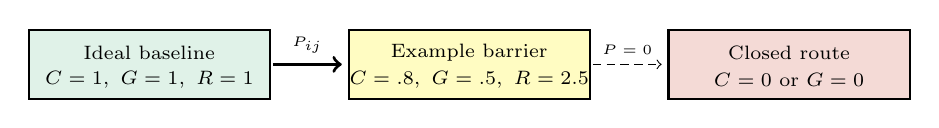
\begin{tikzpicture}[x=1.25cm,y=.8cm, every node/.style={font=\scriptsize}]
  \fill[softgreen] (0,0) rectangle (2.45,1.1);
  \fill[yellow!24] (3.25,0) rectangle (5.70,1.1);
  \fill[hardred] (6.50,0) rectangle (8.95,1.1);
  \draw[thick] (0,0) rectangle (2.45,1.1) (3.25,0) rectangle (5.70,1.1) (6.50,0) rectangle (8.95,1.1);
  \node at (1.225,.73) {Ideal baseline}; \node at (1.225,.31) {$C=1,\ G=1,\ R=1$};
  \node at (4.475,.73) {Example barrier}; \node at (4.475,.31) {$C=.8,\ G=.5,\ R=2.5$};
  \node at (7.725,.73) {Closed route}; \node at (7.725,.31) {$C=0\ \text{or}\ G=0$};
  \draw[->,very thick] (2.48,.55)--(3.18,.55) node[midway,above,font=\tiny] {$P_{ij}$};
  \draw[->,densely dashed] (5.73,.55)--(6.43,.55) node[midway,above,font=\tiny] {$P=0$};
\end{tikzpicture}
\caption{Resistance is a relative movement cost, not a force and not a statement that a cell contains a fixed number of insects.}
\label{fig:resistance}
\end{figure}

\newpage
\section*{3. Exactly how climate and geography enter}
Climate and geography have different jobs.  In the coupled model:
\begin{itemize}\setlength\itemsep{1pt}
\item \textbf{Climate controls establishment:} the local rate is $r_i=rC_i$.  A cell with $C=.4$ gets $40\%$ of the literature-anchored maximum growth rate.
\item \textbf{Climate and terrain control movement:} they multiply to form $H=CG$, then Equation (2) converts $H$ into cell resistance and edge permeability.
\item \textbf{Terrain does not directly kill pressure:} steep/high terrain only slows exchange through $G$.  This avoids claiming that every ridge is impassable.
\end{itemize}
The environmental inputs follow variables repeatedly selected in lanternfly establishment studies---especially dry-quarter temperature, isothermality, cold-quarter precipitation, and elevation \citep{wakie2020,zhao2024}.  $C$ is a normalized WorldClim temperature/moisture factor and $G$ is a normalized elevation-and-slope permeability layer.  Their $0$--$1$ values are \emph{input indices}, not additional physical constants.  A future calibrated species-distribution model should replace these explanatory indices; the present report does not pretend their scores are measured survival probabilities.

The five map modes are controlled comparisons.  Distance diffusion has no growth or resistance; Fisher--KPP sets $C=G=1$ everywhere; Climate applies $C$ to growth and movement; Terrain applies $G$ only to movement; and Climate $+$ Terrain uses the coupled rules above.  Human-assisted jumps are intentionally absent from Equation (1).  They are important in the literature \citep{ladin2023,belouard2025}, but those studies do not supply a transferable continuous jump coefficient for this normalized $u$ field.  Inventing one would violate the stated parameter rule.

\section*{4. Why smaller cells are now higher physics resolution}
The previous interface solved on $1^\circ$ cells and interpolated the result into smaller squares.  The revised solver instead constructs Equation (1) separately at every slider level.  The environmental inputs are remapped to the selected mesh, but the state, neighbor graph, physical distances $d_{ij}$, resistance edges, and annual linear solve all belong to that mesh.

\begin{figure}[h]
\centering
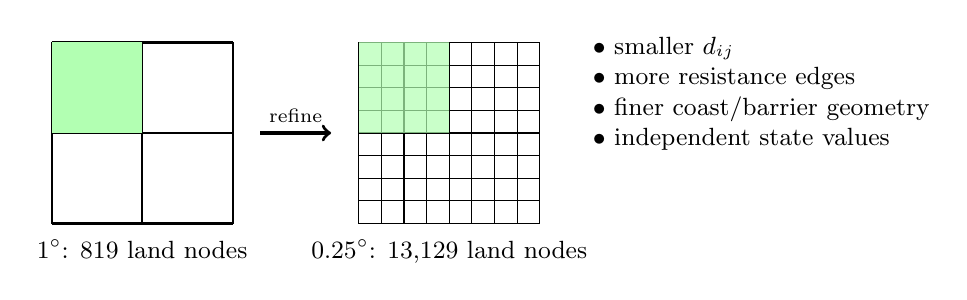
\begin{tikzpicture}[every node/.style={font=\small}]
  \begin{scope}[shift={(0,0)}]
    \draw[step=1.15,thick] (0,0) grid (2.3,2.3);
    \fill[green!30] (0,1.15) rectangle (1.15,2.3);
    \node[below] at (1.15,-.08) {$1^\circ$: 819 land nodes};
  \end{scope}
  \draw[->,very thick] (2.65,1.15)--(3.55,1.15) node[midway,above,font=\scriptsize] {refine};
  \begin{scope}[shift={(3.9,0)}]
    \draw[step=.2875,thin] (0,0) grid (2.3,2.3);
    \fill[green!30,opacity=.7] (0,1.15) rectangle (1.15,2.3);
    \node[below] at (1.15,-.08) {$0.25^\circ$: 13,129 land nodes};
  \end{scope}
  \node[align=left,anchor=west] at (6.75,1.65) {$\bullet$ smaller $d_{ij}$\\$\bullet$ more resistance edges\\$\bullet$ finer coast/barrier geometry\\$\bullet$ independent state values};
\end{tikzpicture}
\caption{The fine mesh contains roughly sixteen times as many land physics nodes.  It is not a subdivision of a rendered coarse column.}
\label{fig:resolution}
\end{figure}

Numerically, each annual update first applies the exact logistic-growth solution in every cell, then solves diffusion implicitly (backward Euler).  This is stable across all four cell sizes without a user-tuned stability factor.  Water-majority cells and the outer domain use no-flux boundaries and remain zero.  Values are stored only for visualization after the solve.

\section*{5. What the result does and does not mean}
A taller cell means more \emph{relative simulated pressure} under the selected mechanism.  It is not a projected lanternfly count, an occupancy probability, or a management recommendation.  The strongest claim is narrower: with the cited growth and spread scales held fixed, the app shows how a resistance surface redirects and slows a Fisher--KPP-like front, and it now resolves that mechanism more finely when the cell-size slider is moved left.

\vspace{-0.3em}
\setlength{\parskip}{0pt}
\begin{thebibliography}{9}\tiny
\setlength{\itemsep}{0pt}
\setlength{\parsep}{0pt}
\bibitem{fisher1937} Fisher, R.A. (1937). The wave of advance of advantageous genes. \emph{Annals of Eugenics}, 7, 355--369.
\bibitem{ladin2023} Ladin, Z.S. et al. (2023). Human-mediated dispersal drives the spread of the spotted lanternfly. \emph{Scientific Reports}, 13, 1098. \href{https://doi.org/10.1038/s41598-022-25989-3}{doi:10.1038/s41598-022-25989-3}.
\bibitem{belouard2025} Belouard, N. et al. (2025). A method to quantify jump dispersal of invasive species. \emph{NeoBiota}, 98, 319--334. \href{https://doi.org/10.3897/neobiota.98.147310}{doi:10.3897/neobiota.98.147310}.
\bibitem{ruzzier2025} Ruzzier, E. et al. (2025). Predicting the global distribution and invasion scenarios of the Spotted Lanternfly. \emph{NeoBiota}, 103, 267--298. \href{https://doi.org/10.3897/neobiota.103.154246}{doi:10.3897/neobiota.103.154246}.
\bibitem{wakie2020} Wakie, T.T. et al. (2020). Establishment risk of \emph{Lycorma delicatula} in the United States and globally. \emph{Journal of Economic Entomology}, 113, 306--314. \href{https://doi.org/10.1093/jee/toz259}{doi:10.1093/jee/toz259}.
\bibitem{zhao2024} Zhao, Z., Yang, L. \& Chen, X. (2024). Globally suitable areas for \emph{Lycorma delicatula} based on an optimized Maxent model. \emph{Ecology and Evolution}, 14, e70252. \href{https://doi.org/10.1002/ece3.70252}{doi:10.1002/ece3.70252}.
\end{thebibliography}

\end{document}
